
\section{Overview}

For some time, there has been a need for a \cpp\ class embodying the
information contained in the Review of Particle Properties\cite{pdg}.
We have written HepPDT to fill this need.  
HepPDT allows access
to particle name, particle ID, charge, nominal mass,  total width,
spin information, color information, constituent particles, and
decay mode information.
HepPDT is designed to be used by StdHepC++\cite{stdhep}
or any Monte Carlo generated particle class. 
Generated particles will contain a
pointer to the particle data information found in the HepPDT
particle data table.  
HepPDT also has simple mechanisms to enable customized decay chains.

\subsection{HepPDT Design}

HepPDT has been designed to be used by any Monte Carlo particle generator
or decay package.  It contains only generic particle attributes.
In principle, all information which can be found in
the Review of Particle Properties\cite{pdg} can be encapsulated in HepPDT.
HepPDT contains particle information such as charge and nominal mass
as well as decay mode information.  This information is contained
in a table which is accessed by a particle ID number.  This ID number
is defined according to the Particle Data Group's
Monte Carlo numbering scheme\cite{newscheme}.  

HepPDT may be used alone or as part of the StdHepC++\cite{stdhep} package.
StdHepC++ provides a standard generated particle class which can be used
to communicate among various Monte Carlo generators and decay packages.
A StdHep particle contains momentum information, generated mass, 
information about its generated decay, and 
a pointer to the appropriate HepPDT particle data.

Decay information is a crucial part of the particle data in HepPDT.
Standard decay information is a list of allowed decay channels with
associated branching fractions, decay model names and decay model code.  
There may also be
extra information needed by the decay model (\eg, helicity).
A mechanism is provided so that the decay model code can be accessed
using the decay data information instead of needing to use
a series of if statements based on the decay model name.
In addition, users often need the ability to ``force'' a \
particle to decay in a certain way.
To do this, you must provide custom decay information.  Often this information
involves the entire decay chain (\eg, $D^{*+} \rightarrow D^0 \pi^+, 
D^0 \rightarrow K^- \pi^+$).  The design allows the generated
particle to have a pointer to a custom DecayData object.  
If this pointer is non-null,the pointed-to
object overrides the DecayData associated with the generated
particle's ParticleData. 
To customize the decay chain, the user may create
particle aliases which use other special DecayData objects.

Methods are provided to create ParticleDataTable objects from
Pythia, Herwig, Isajet, QQ, and EvtGen decay information.  Methods
are also provided to facilitate creation of custom particle and
decay information.  A ParticleDataTable object may be created from
multiple information sources.

The design requires that ParticleDataTable objects must be fully created
before they are used.  Multiple data tables are allowed.  Although
potentially dangerous, we recognize that this is also a powerful option.

Figure~\ref{fig:a} shows the interactions of the basic classes.

\begin{figure}
  \epsfig {file=HepPDT-class.eps, width=18cm }
\caption{HepPDT Classes: 
Particle information is accessed by a pointer to ParticleData from any
Monte Carlo generated particle.  
CommonParticleData contains particle information such as mass, charge,
and total width.  Decay information is found in DecayData.
The ParticleDataTable contains a map of ParticleData objects,
referenced by ParticleID, as well as lists of CommonParticleData and DecayData.
ParticleData has indices to CommonParticleData and DecayData, as well as
methods to access all relevant information.  
The DecayModelFactory is used to create DecayModelBase objects
which are derived from user DecayModel classes. }
\label{fig:a}
\end{figure}

\subsection{HepPDT Classes}

The ParticleDataTable class contains a map of ParticleData
which is keyed on the ParticleID class.  Particle ID aliases can be used
to add custom DecayData.  ParticleDataTable also contains lists
of CommonParticleData and DecayData.

The ParticleID
class can be used to retrieve all the information that is implied 
in the particle ID (\eg, charge and quark content).   Boolean methods
(such as isMeson, isBaryon, hasBottom, and hasTop) are provided
for ease of searching for various types of particles.

The ParticleData class has iterators into the lists
of CommonParticleData and DecayData.   CommonParticleData is extensible
and includes particle name, particle ID, charge,
mass, total width with cutoffs, spin information, color information, 
and constituent particles (\eg, quark content).  
This class is not templated.

The DecayData class is a collection of DecayChannels.
A generated particle may use the DecayData information from the
ParticleDataTable entry or it may use a customized DecayData that
allows, for instance, only a single DecayChannel.
Users may add customized DecayData objects to the ParticleDataTable.

Each DecayChannel has a collection of decay channel products
(which are pointers to ParticleData), a decay name, a branching fraction,
an optional vector of extra decay model parameters, and a 
pointer to DecayModelBase.  We recognize that other information, such
as helicity, may be needed by a particular DecayChannel object.
Because there are many options, 
this information is stored as a vector of doubles.  

\section { Particle Numbering Scheme }

A basic particle numbering scheme was proposed by the Particle Data
Group in 1988\cite{pdg88}.  
Practical application of this scheme exposed some limitations.
After consultation\cite{knowles}, the scheme was revised to 
better match the practice of program authors.  The revised scheme
includes numbering states by orbital and radial quantum numbers
to allow systematic inclusion of quark model states which are
as yet undiscovered.  The new scheme also includes numbering for
hypothetical particles such as SUSY particles.

Because the old PDG convention allowed a fair amount of room for 
interpretation,
the implementation tended to have minor variations among packages.
With the new scheme, there is much less variation, but occasional differences
remain.  

The standard particle numbering scheme is explained in full detail in
reference \cite{newscheme}.

Quarks, leptons, guage bosons, Higgs, and similar particles are assigned
numbers between 1 and 80.  
Numbers 81-100 are for generator specific use.
Any particle with an ID of 100 or less is considered a "fundamental" particle.
The list of fundamental particles is in Appendix \ref{elem}.

The PDG numbering algorithm for composite particles uses a signed 7 
digit number for each particle:  $\pm nn_rn_Ln_{q_1}n_{q_2}n_{q_3}n_J$.
$n_{q_{1-3}}$ are quark numbers used to specify the quark content.
The rightmost digit, $n_J$ = 2J + 1, gives the total spin of the composite particle.
The scheme does not cover particles of total spin $J>4$.
The fifth digit, $n_L$, is reserved to distinguish mesons of the
same total ($J$) but different spin ($S$) and orbital ($L$)
angular momentum quantum numbers.
The sixth digit, $n_r$, is used to label mesons radially excited
above the ground state.
Many states appearing in the PDG meson listing do not yet have definite
$q\bar q$ model assignments.  For these states, $n_{q_{2-3}}$
and $n_J$ are assigned according to the state's most likely flavors
and spin.  Within these groups $n_L=0,1,2,\dots$ is used to distinguish
states of increasing mass. These states are flagged with $n=9$.
The numbering scheme does not extend to baryons with $n>0$, $n_r>0$, or $n_L>0$.
Digits $n_{q_2}$ and $n_{q_3}$ are used for mesons, with $n_{q_1}$ = 0.
Digits $n_{q_1}$, $n_{q_2}$, and $n_{q_3}$ are used for baryons.
Digits $n_{q_1}$ and $n_{q_2}$ are used for diquarks, with $n_{q_3}$ = 0. 
(A list of diquark states is in Appendix \ref{elem}.)  
A negative number indicates an antiparticle.  
The states are generally listed in order of increasing mass.  
$K_L^0$ and $K_S^0$ are exceptions.  Their assigned
identification numbers are 130 and 310, respectively.

SUSY particles are indicated with $n=1$ for right-handed particles or $n=2$
for left-handed particles.  Technicolor states have $n=3$.
Excited (composite) quarks and leptons are identified by setting $n=4$.
Other exotic particles have $n n_r=51$.

The new numbering scheme attemts to list all states needed by the
Monte Carlo generators.  Appendix \ref{meson}
contains a full list of meson states and their ID numbers, up through the
top quark states.   

The baryon $\Xi$ and $\Omega$ states for charmed
and heavier quarks require special consideration.  
Three spin 1/2 states are recognized
for cxy, bxy, etc., where x and y are lighter, non-identical quarks.
The non-primed states are antisymmetric under interchange of the lighter quarks.
and the primed states are symmetric.  The numbering for these states is 
explicitly stated in the new numbering scheme.
Appendix \ref{baryon} contains a full list of the baryon states.

HepPDT uses an ad-hoc numbering scheme for ions.  
Ion numbers are $FAAAZZZ00n_J$, where F = 1 and flags this
as an ion.  AAA, and ZZZ are the ion's A and Z respectively.
The first digit, $n_J$, contains the total spin as $n_J$ = 2J + 1.

\subsection { Generator Numbering Schemes }

The Isajet particle identification algorithm uses a signed four digit
number: $\pm$MLKJ.  M, L, and K are quarks and J is the spin.  A negative
number indicates the antiparticle, and is meant to associate with the
lightest quark.  For mesons, M = 0, and for diquarks, K = 0.

Pythia, Herwig, EvtGen, and QQ use the PDG algorithm in addition to internal
compressed numbering schemes.
Although the latest implementations of Pythia, Herwig, and QQ conform closely
to the new numbering scheme, some differences remain.

Isajet, Herwig, and Pythia contain the possibility of
defining fourth family states. 

\subsection { ParticleID }

The HepPDT::ParticleID class  
provides methods to return all the information
which can be extracted or inferred from the particle ID (PID).
It is expected that any 7 digit number used as a PID will adhere to the 
rules of the Monte Carlo Particle Numbering Scheme published by the
PDG.\cite{pdg}

The ParticleID class considers any particle with 
an ID less than 100 a "fundamental" particle.

In most cases, a user can define particles not already in the
Particle Data Table without needing to extend the numbering scheme.
A previously unknown particle can be assigned a valid PID by
following the rules in the "Review of Particle Physics".\cite{pdg}

If the user wishes to force the decay chain 
$D^* \rightarrow D^0 \pi^0, D^0 \rightarrow K^- \pi^+ \pi^0 \pi^0$,
a user might define a special $D^0$ which only decays to 
$K^- \pi^+ \pi^0 \pi^0$, leaving any $D^0$ produced elsewhere to decay normally.
The PID for a normal $D^0$ is 421.  The PID for the special $D^0$
might be 6000421.   This new PID might be used in several different jobs
for $D^0$ particles with different forced decay modes.
(EvtGen defines these special particles as aliases in the decay table.
The TableBuilder class handles the aliases appropriately without needing
to create a new PID for the particle alias.)

\begin{center}
\begin{tabular}{ll}
 & ParticleID( int pid = 0 ); \\
 & ParticleID( const ParticleID \& orig );  \\
 & ParticleID \& operator=( const ParticleID \& );  \\
void & swap( ParticleID \& other );  \\
bool  & operator $<$  ( ParticleID const \& other ) const;  \\
bool   &operator == ( ParticleID const \& other ) const;  \\
 \\
int   &  pid( )        const;  \\
int & abspid( )        const;  \\
 \\
bool & isValid( )   const; \\
bool & isMeson( )   const;\\
bool  & isBaryon( )  const;\\
bool  & isDiQuark( ) const;\\
bool & isHadron( )  const; \\
bool & isLepton( )  const; \\
bool & isNucleus( )  const; \\
 \\
bool & hasUp( )      const; \\
bool & hasDown( )    const;\\
bool & hasStrange( ) const;\\
bool & hasCharm( )   const;\\
bool & hasBottom( )  const;\\
bool & hasTop( )     const;\\
\multicolumn{2}{l} {\bf In practice, it is better to query the ParticleData class
for quark content.} \\
 \\
int  & jSpin( )        const; \\
int  & sSpin( )        const;\\
int  & lSpin( )        const; \\
int & fundamentalID( ) const; \\
Quarks & quarks( ) const; \\
int & threeCharge( ) const; \\
int & A( ) const;\\
int & Z( ) const;\\
unsigned short & digit(location) const; \\
\end{tabular}
\end{center}

\subsection { Translating Particle ID's }

The header ParticleID.hh defines a number of free functions which can
be used to translate between generator and HepPDT numbering schemes.

\begin{center}
\begin{tabular}{ll}
int & translatePythiatoPDT( const int pythiaID ); \\
int & translateIsajettoPDT( const int isajetID ); \\
int & translateHerwigtoPDT( const int herwigID); \\
int & translateQQtoPDT( const int qqID); \\
int & translateGeanttoPDT( const int geantID); \\
int & translatePDGtabletoPDT( const int pdgID); \\
int & translateEvtGentoPDT( const int evtGenID ); \\
 \\
int & translatePDTtoPythia( const int pid ); \\
int & translatePDTtoIsajet( const int pid ); \\
int & translatePDTtoHerwig( const int pid ); \\
int & translatePDTtoQQ( const int pid ); \\
int & translatePDTtoGeant( const int pid ); \\
int & translatePDTtoPDGtable( const int pid ); \\
int & translatePDTtoEvtGen( const int pid ); \\
\end{tabular}
\end{center}


\section { Particle Properties }

Particle data information is stored in HepPDT::ParticleDataTable, 
which is a map of HepPDT::ParticleData objects
that are referenced by HepPDT::ParticleID. 
The design envisions that generated particles will contain links
to the relevant  HepPDT::ParticleData object.

\subsection { Reading Particle Data information }

HepPDT can accept particle data information from a variety of sources.
To fill HepPDT::ParticleDataTable, 
the user creates an empty ParticleDataTable object
and then calls HepPDT::TableBuilder methods to read the information 
from an input stream.
Information may be read from as many input streams as desired.
In case of conflicts, previous information will be overwritten.
All information is kept in temporary objects until the TableBuilder destructor
is called.  
The TableBuilder destructor then creates the ParticleData objects owned
by ParticleDataTable.  

The following code fragment reads Pythia input from a flat file.
Examples reading input from other sources are in Appendix \ref{readdata} 
and also in the example subdirectory. 

\begin{verbatim}
#include <fstream>

#include "HepPDT/TableBuilder.hh"
#include "HepPDT/ParticleDataTable.hh"
#include "HepPDT/TempParticleData.hh"

    const char infile[] = "data/pythia.tbl";
    // open input file
    std::ifstream pdfile( infile );
    if( !pdfile ) { 
      std::cerr << "cannot open " << infile << std::endl;
      exit(-1);
    }
    // construct empty PDT
    HepPDT::ParticleDataTable datacol( "Pythia Table" );
    {
        // Construct table builder
        HepPDT::TableBuilder  tb(datacol);
	// read the input - put as many here as you want
        if( !addPythiaParticles( pdfile, tb ) ) 
	      { std::cout << "error reading pythia file " << std::endl; }
    }	// the tb destructor fills datacol
\end{verbatim}

The Particle Data Group provides a table of particle masses and widths for known
particles.  This table,  pdg\_mass.tbl, is distributed with the HepPDT package.
This information is also available from specific generators, often as
flat files.  HepPDT contains 

\subsection { Accessing Particle Data information }

The following code fragment accesses pion and muon information.
Refer to the Appendices for a listing of particle ID numbers.
\begin{verbatim}
    std::ofstream wpdfile( outfile );
    HepPDT::ParticleDataTable db( "my Table" );
    ......
    HepPDT::ParticleData * pd = datacol.particle( HepPDT::ParticleID(111) );
    pd->write(wpdfile);
    double mumass = datacol.particle( HepPDT::ParticleID(13) )->mass();
\end{verbatim}

In principle, all information in the PDG may be obtained from ParticleData
access methods.

\begin{center}
\begin{tabular}{ll}
  std::string const \&         & name()        const;  \\    
  ParticleID                  & ID()          const; \\
  int                         & pid( )        const; \\
  double                      & charge()      const; \\
  double                      & color()       const; \\
  SpinState                   & spin()        const; \\
  Measurement                 & mass()        const; \\
  Measurement                 & totalWidth()  const; \\
  Measurement                 & lifetime()    const; \\
  int                         & numConstituents() const; \\
   Constituent          & constituent( unsigned int i ) const; \\
   ParticleID           & constituentParticle( unsigned int i ) const; \\
  ResonanceStructure const *  & resonance()   const; \\
 \\
  bool & isMeson( )   const; \\
  bool & isBaryon( )  const; \\
  bool & isDiQuark( ) const; \\
  bool & isHadron( )  const; \\
  bool & isLepton( )  const; \\
  bool & isNucleus( ) const; \\
  bool & hasUp()      const; \\
  bool & hasDown()    const; \\
  bool & hasStrange() const; \\
  bool & hasCharm()   const; \\
  bool & hasBottom()  const; \\
  bool & hasTop()     const; \\
 \\
  int                  & numDecayChannels() const; \\
  bool                 & isStable()         const; \\
  DecayChannel  & channel( int i )    const; \\
  DDID   & getDecayData()            const; \\
  CPDID  & getCommonParticleData()   const; \\
   \\
   void & write( std::ostream \& os ) const; \\
\end{tabular}
\end{center}

\subsection{ The Measurement Class }

Some tables contain errors on mass and width values.
To keep this error information available, we wrote a simple HepPDT::Measurement
class which contains a double value and a double error on the value.
If you reference it with a double, Measurement returns the value.

\begin{center}
\begin{tabular}{ll}
 & Measurement( double value, double sigma ); \\
 & Measurement( const Measurement \& orig );  \\
 & Measurement \& operator=( const Measurement \& );  \\
void & swap( Measurement \& other );  \\
bool  & operator $<$  ( Measurement const \& other ) const;  \\
bool   & operator == ( Measurement const \& other ) const;  \\
   double  &  value()  const;\\
   double   & sigma()  const;\\
   operator & double() const;\\
\end{tabular}
\end{center}

\section{Use of Templates}

Decay methods are, by definition, outside the scope of 
HepPDT.  However, the user may wish to be able to call 
decay methods from DecayChannel.

DecayModelBase is the mechanism that allows
the user to invoke an actual decay method from this class.
Because the decay method must
know what kind of generated particle will be created,
DecayModelBase is a class \textit{template}, parameterized on the
type of particle to be generated. Because of the need to allow the
user freedom of choice for this generated particle class, many
related abstractions in this model are also class templates. In
each case, a typedef is provided to allow users who do not need
this degree of flexibility to ignore it. These typedefs also stand
as an example for those groups who wish to standardize upon a
common type for the generated particles.

\section{Decay Model Factory}

In order to allow users to ``plug-in'' new decay models
(subclasses of DecayModelBase), without requiring recompilation of
the entire library, we provide the class template
DecayModelFactory, and a simple means by which user-written decay
models will be automatically registered for creation, when
requested by a DecayData object. This is done by the common
technique of having each decay model register (at static
initialization time) a function object that is used to create
instances of that decay model.

\section{Conclusions}

HepPDT provides access to all useful particle data properties
and is designed to be used with any generated particle.    
It also contains
a factory to allow the user to directly access decay model code
instead of needing to use a lookup table or series of if
statements based on the decay model name.  HepPDT will be part of the
StdHepC++ package in CLHEP\cite{clhep} and is available now at 
http://www-pat.fnal.gov/stdhep/c++/.

